\chapter{A Mecânica dos Sólidos: tensão, deformação e deslocamento}

A Mecânica dos Sólidos é parte da física que estuda o comportamento de objetos sólidos sobre carregamentos, aplicando métodos analíticos para determinar suas características de resistência, rigidez e estabilidade. Seu conteúdo é notório por ser fundamental para grande parte da vida dos engenheiros, sendo mecânicos, civis ou mesmo eletricistas, ao lado de outras áreas também tão fundamentais, como Mecânica dos Fluidos e Termodinâmica. Sua aplicação é voltada ao projeto de estruturas a fim de que cumpram determinadas exigências, sejam tanto de deformação máxima, capacidade de carga e peso, como também de economia de materiais. E, por meio de ferramentas matemáticas, estuda os efeitos de tensão e deformação no interior de corpos sólidos. \cite{popov}

Este capítulo aborda os seguintes temas de Mecânica dos Sólidos, relevantes para o desenvolvimento inicial do módulo PHILLIPO.jl voltado à análise de estruturas elásticas sobre carregamentos contantes:
\begin{enumerate}
    \item tensão;
    \item deslocamento e deformação;
    \item estado de tensão;
    \item lei de Hooke generalizada;
    \item modelo de viga de Euler-Bernoulli;
    \item critérios de tensão máxima admissível.
\end{enumerate}

Todos os conceitos deste capítulo seguem as definições do livro de \citeauthor{popov}: \emph{Engineering Mechanics of Solids}, de 1990.

\section{Tensão}

Um corpo sólido se deforma quando submetido a carregamentos externos, distribuindo essas cargas ao longo de sua geometria. Tensão define a grandeza dessa distribuição agindo sobre áreas infinitesimais, de modo que qualquer secção do corpo revele forças internas que estejam em equilíbrio entre si, e que sejam balanceadas pelo carregamentos externos. Essas forças, geralmente, variam ao longo do corpo, como também, dependem do plano de seção. E, devido a sua forma vetorial, é conveniente que sejam decompostas em parcelas tangenciais e normais à seção. \cite{popov}

Seja um corpo $\bm{K}$, sólido, em equilíbrio e de geometria qualquer, submetido a forças externas $\vec{F}$, e as seções $S_{1,2,3}$ planos de corte através de esse corpo, ortogonais entre si, em que atuam as forças internas $\vec{P}$:

\begin{figure}
    \centering
    \caption{Forças internas: seção em um sólido qualquer}
    \begin{subfigure}[b]{\textwidth}
        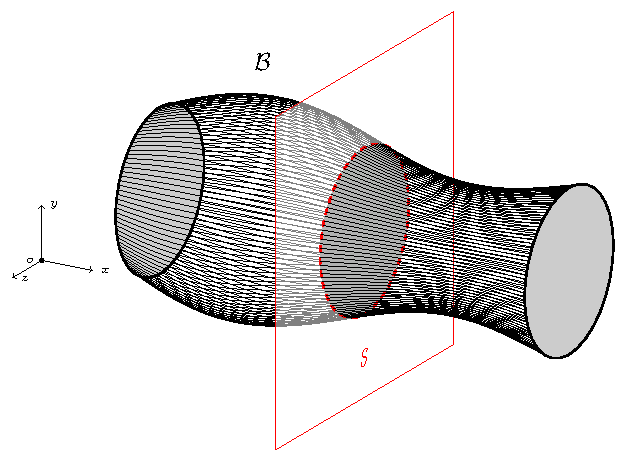
\includegraphics[scale=0.7]{Figuras/forcas_internas_2.pdf}
        \caption{$ $}
        \label{fig:forcas_internas_1}
    \end{subfigure}
    \hfill
    \begin{subfigure}[b]{\textwidth}
        \centering
        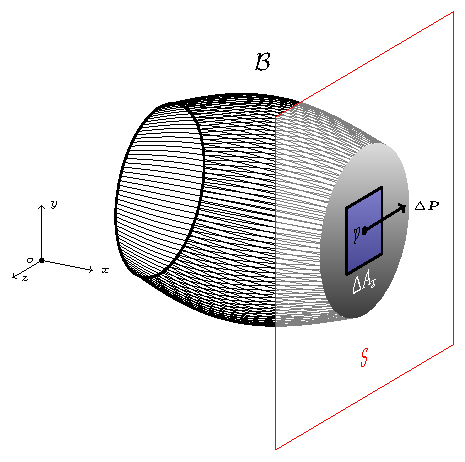
\includegraphics[scale=0.7]{Figuras/forcas_internas_1.pdf}
        \caption{$ $}
        \label{fig:forcas_internas_2}
    \end{subfigure}
    \hfill
    \begin{subfigure}[b]{\textwidth}
        \centering
        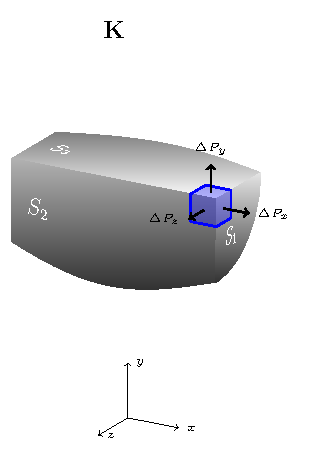
\includegraphics[scale=0.7]{Figuras/forcas_internas_3.pdf}
        \caption{$ $}
        \label{fig:forcas_internas_3}
    \end{subfigure}
       \label{fig:forcas_internas}
\end{figure}

em que $\Delta\vec{P}$ simboliza a força equivalente agindo  sobre uma aréa $\Delta A$ discretizada de $S$.
